\documentclass[]{article}

%environnement
\usepackage[letterpaper,margin=1in]{geometry}
\usepackage[utf8]{inputenc}
\usepackage{fontspec}
\usepackage[english]{babel}
\usepackage[parfill]{parskip}
\usepackage[style=ieee,backend=bibtex]{biblatex} %gestion bib
\usepackage{listings}
\usepackage{hyperref}
\usepackage[toc,acronym]{glossaries}
\usepackage[framemethod=TikZ]{mdframed} 
\usepackage{todonotes}
\usepackage[section]{placeins}
\hypersetup{
	pdftitle={},
	pdfborder={0 0 0}, %epaisseur box
	pdfauthor={Thomas LUINAUD},
}
\usepackage{tikz,tkz-tab}%package pour les tableaux de variations et de signes%
\usetikzlibrary{babel}
\usepackage{modules/tikzNetwork}
\usepackage{circuitikz}
\usetikzlibrary{positioning, automata, graphs, trees, fit, arrows.meta, shapes}
\usetikzlibrary{backgrounds,patterns,matrix,calc,shadows,plotmarks, circuits.logic.US}
\usetikzlibrary{decorations}
\usepackage{multirow}
\usepackage{modules/moeptikz}
%\usepackage{tabularx}
 %this file contains shape declaration and macro that define 
 %basic computer science shape for Hardware design.
 %this file should be include in the preamble
 
 \catcode`@=11

\pgfkeys{%
  /pgf/logicalbloc io north/.initial=5,
%  /pgf/logicalbloc io south/.initial=10,
%  /pgf/logicalbloc io east/.initial=10,
  /pgf/logicalbloc io west/.initial=10,
  /pgf/logicalbloc io north spacing/.initial=0.15cm,
%  /pgf/logicalbloc io south spacing/.initial=0.25cm,
%  /pgf/logicalbloc io east spacing/.initial=0.25cm,
  /pgf/logicalbloc io west spacing/.initial=0.20cm
}
\def\maxpins{100}


%stdChip
\pgfdeclareshape{logicalbloc}{
	\savedanchor\centerpoint{% 
		\pgf@x=.5\wd\pgfnodeparttextbox%
		\pgf@y=.5\ht\pgfnodeparttextbox%
		\advance\pgf@y by-.5\dp\pgfnodeparttextbox%
	  }
	  \anchor{center}{\centerpoint}
	  
	  \saveddimen\height{%
		\pgfmathsetlength\pgf@x{(\pgfkeysvalueof{/pgf/logicalbloc io west}+1)*\pgfkeysvalueof{/pgf/logicalbloc io west spacing}}%
	  }
	  \saveddimen\width{%
		\pgfmathsetlength\pgf@y{(\pgfkeysvalueof{/pgf/logicalbloc io north}+1)*\pgfkeysvalueof{/pgf/logicalbloc io north spacing}}%
	  }
	  \saveddimen{\yspacing}{\pgfmathsetlength\pgf@x{\pgfkeysvalueof{/pgf/logicalbloc io west spacing}}}	  
	  \saveddimen{\xspacing}{\pgfmathsetlength\pgf@y{\pgfkeysvalueof{/pgf/logicalbloc io north  spacing}}}
	  
	  \backgroundpath{%
		\pgfpathrectanglecorners{\pgfpointadd{\centerpoint}{\genbottomleftpoint}}%
		{\pgfpointadd{\centerpoint}{\gentoprightpoint}}%
	  }
 

	  \pgfmathloop%
	  \ifnum\pgfmathcounter>\maxpins\relax% 
	  \else%
		% Need to expand \pgfmathcounter
		\edef\marshal{\noexpand\anchor{io east \pgfmathcounter}}%
		\expandafter\marshal\expandafter{\expandafter\chippinanchorright\expandafter{\pgfmathcounter}}%
	  \repeatpgfmathloop%
	  
	  \pgfmathloop%
	  \ifnum\pgfmathcounter>\maxpins\relax% 
	  \else%
		% Need to expand \pgfmathcounter
		\edef\marshal{\noexpand\anchor{io north \pgfmathcounter}}%
		\expandafter\marshal\expandafter{\expandafter\chippinanchorupper\expandafter{\pgfmathcounter}}%
	  \repeatpgfmathloop%
	  
	  \pgfmathloop%
	  \ifnum\pgfmathcounter>\maxpins\relax% 
	  \else%
		% Need to expand \pgfmathcounter
		\edef\marshal{\noexpand\anchor{io south \pgfmathcounter}}%
		\expandafter\marshal\expandafter{\expandafter\chippinanchorbottom\expandafter{\pgfmathcounter}}%
	  \repeatpgfmathloop%
	  
	  \pgfmathloop%
	  \ifnum\pgfmathcounter>\maxpins\relax% 
	  \else%
		% Need to expand \pgfmathcounter
		\edef\marshal{\noexpand\anchor{io west \pgfmathcounter}}%
		\expandafter\marshal\expandafter{\expandafter\chippinanchorleft\expandafter{\pgfmathcounter}}%
	  \repeatpgfmathloop%
}

\def\genbottomleftpoint{%
%	\pgfmathsetlength{pgf@xb}{(\pgfkeysvalueof{/pgf/logicalbloc io north}+1)*\pgfkeysvalueof{/pgf/logicalbloc io north spacing}}%
%	\pgfmathsetlength{pgf@yb}{(\pgfkeysvalueof{/pgf/logicalbloc io west}+1)*\pgfkeysvalueof{/pgf/logicalbloc io west spacing}}%
%	\setlength{\pgf@xa}{1cm}
%	\setlength{\pgf@ya}{1cm}
%	\if \pgf@xb<\pgf@xa
%		\if \pgf@yb<\pgf@ya
%			\pgfpoint{-0.5cm}{-0.5cm}
%		\else
%			\pgfpoint{-0.5cm}{-(\pgfkeysvalueof{/pgf/logicalbloc io west}+1)*\pgfkeysvalueof{/pgf/logicalbloc io west spacing}/2}
%		\fi
%	\else
%		\if \pgf@yb<\pgf@ya
%			\pgfpoint{-(\pgfkeysvalueof{/pgf/logicalbloc io north}+1)*\pgfkeysvalueof{/pgf/logicalbloc io north spacing}/2}{-0.5cm}
%		\else
			\pgfpoint{-((\pgfkeysvalueof{/pgf/logicalbloc io north}+1)*\pgfkeysvalueof{/pgf/logicalbloc io north spacing})/2}{-((\pgfkeysvalueof{/pgf/logicalbloc io west}+1)*\pgfkeysvalueof{/pgf/logicalbloc io west spacing})/2}
%		\fi
%	\fi
}
\def\gentoprightpoint{%
%	\if {\pgfkeysvalueof{/pgf/logicalbloc io west} < \pgfkeysvalueof{/pgf/logicalbloc io east}}
%		\setlength{\pgf@xc}{1cm}
%	\else
%		\setlength{\pgf@xc}{1cm}
%	\fi
%	\if
%		\setlength{\pgf@xc}{1cm}
%	\else
%		\setlength{\pgf@xc}{1cm}
%	\fi
%	\pgfmathsetlength{pgf@xb}{(\pgfkeysvalueof{/pgf/logicalbloc io north}+1)*\pgfkeysvalueof{/pgf/logicalbloc io north spacing}}%
%	\pgfmathsetlength{pgf@yb}{(\pgfkeysvalueof{/pgf/logicalbloc io west}+1)*\pgfkeysvalueof{/pgf/logicalbloc io west spacing}}%
%	\setlength{\pgf@xa}{1cm}
%	\setlength{\pgf@ya}{1cm}
%	\if \pgf@xb<\pgf@xa
%		\if \pgf@yb<\pgf@ya
%			\pgfpoint{0.5cm}{0.5cm}
%		\else
%			\pgfpoint{0.5cm}{(\pgfkeysvalueof{/pgf/logicalbloc io west}+1)*\pgfkeysvalueof{/pgf/logicalbloc io west spacing}/2}
%		\fi
%	\else
%		\if \pgf@yb<\pgf@ya
%			\pgfpoint{(\pgfkeysvalueof{/pgf/logicalbloc io north}+1)*\pgfkeysvalueof{/pgf/logicalbloc io north spacing}/2}{0.5cm}
%		\else
			\pgfpoint{((\pgfkeysvalueof{/pgf/logicalbloc io north}+1)*\pgfkeysvalueof{/pgf/logicalbloc io north spacing})/2}{((\pgfkeysvalueof{/pgf/logicalbloc io west}+1)*\pgfkeysvalueof{/pgf/logicalbloc io west spacing})/2}
%		\fi
%	\fi
}


\def\genpointbottom#1{
\pgfpoint{(\pgfkeysvalueof{/pgf/logicalbloc io north}+1)*\pgfkeysvalueof{/pgf/logicalbloc io north spacing}/2-#1*\xspacing}{-(\pgfkeysvalueof{/pgf/logicalbloc io west}+1)*\pgfkeysvalueof{/pgf/logicalbloc io west spacing}/2}
}

\def\chippinanchorbottom#1{%
	  % When this macro is called,
	  % \centerpoint, \height and \chipspacing will be defined.
	  %\pgfpointadd{\centerpoint}{\pgfpoint{\width/2-#1*\xspacing}{-\height/2}}%
	  \pgfpointadd{\centerpoint}{\genpointbottom{#1}}%
}

\def\genpointupper#1{
\pgfpoint{(\pgfkeysvalueof{/pgf/logicalbloc io north}+1)*\pgfkeysvalueof{/pgf/logicalbloc io north spacing}/2-#1*\xspacing}{(\pgfkeysvalueof{/pgf/logicalbloc io west}+1)*\pgfkeysvalueof{/pgf/logicalbloc io west spacing}/2}
}

\def\chippinanchorupper#1{%
	  % When this macro is called,
	  % \centerpoint, \height and \chipspacing will be defined.
	  \pgfpointadd{\centerpoint}{\genpointupper{#1}}%
}

\def\genpointleft#1{
\pgfpoint{-(\pgfkeysvalueof{/pgf/logicalbloc io north}+1)*\pgfkeysvalueof{/pgf/logicalbloc io north spacing}/2}{(\pgfkeysvalueof{/pgf/logicalbloc io west}+1)*\pgfkeysvalueof{/pgf/logicalbloc io west spacing}/2-#1*\yspacing}
}

\def\chippinanchorleft#1{%
	  % When this macro is called,
	  % \centerpoint, \height and \chipspacing will be defined.
	  \pgfpointadd{\centerpoint}{\genpointleft{#1}}%
}

\def\genpointright#1{
\pgfpoint{(\pgfkeysvalueof{/pgf/logicalbloc io north}+1)*\pgfkeysvalueof{/pgf/logicalbloc io north spacing}/2}{(\pgfkeysvalueof{/pgf/logicalbloc io west}+1)*\pgfkeysvalueof{/pgf/logicalbloc io west spacing}/2-#1*\yspacing}
}
\def\chippinanchorright#1{%
	  % When this macro is called,
	  % \centerpoint, \height and \chipspacing will be defined.
	  \pgfpointadd{\centerpoint}{\genpointright{#1}}%
}

\catcode`@=12
\usepackage{cancel}%package pour barrer et simplifier%
\usepackage{amsmath}%matrice%
\usepackage{stmaryrd}
\usepackage{textcomp}
\usepackage{pstricks}
\usepackage{pdftricks, pstricks-add}
\usepackage{pgfplots}
\usepackage{caption}
\usepackage{subfig}
\usepackage{pdfpages}
	
\hyphenation{contien-nent}

\usepackage[nounderscore]{syntax}
\newlength\grammarLongest
\newlength\grammarLeftMargin
\makeatletter
\newenvironment{grammarC}[1]{%
\list{}{%
\settowidth\grammarLongest{#1}
\setlength\grammarLeftMargin{\dimexpr0.5\linewidth-0.5\grammarLongest}
\labelwidth\grammarindent%
\leftmargin\dimexpr\grammarindent+\grammarLeftMargin\relax%
\advance\grammarindent\labelsep
\itemindent\z@%
\listparindent\z@%
\parsep\grammarparsep%
}%
\let\\\@normalcr
\syntaxShortcuts\relax\relax%
\def\alt{\\\llap{\textbar\quad}}%
\def\gr@setpar{%
\def\par{%
\parshape\@ne\@totalleftmargin\linewidth%
\@@par%
\catcode`\<12%
\everypar{%
\everypar{}%
\catcode`\<\active%
\gr@implitem%
}%
}%
}%
\gr@setpar%
\par%
\let\gr@leftsq\[%
\let\gr@rightsq\]%
\def\gr@endsyntdiag]{\end{syntdiag}\gr@setpar\par}%
\def\[{\@ifnextchar[{\begin{syntdiag}\@gobble}\gr@leftsq}%
\def\]{\@ifnextchar]\gr@endsyntdiag\gr@rightsq}%
}{%
\@newlistfalse%
\everypar{}%
\endlist%
}
\makeatother
\usepackage{varwidth}

\usepackage{tabularx}
\usepackage{csvsimple}
\usepackage{float}
\usepackage{amssymb}
\usepackage[linesnumbered,lined, french, frenchkw, figure, noend]{algorithm2e}

\newcommand{\inputFig}[2]{\IfFileExists{#1}{\input{#1}}{\missingfigure[figheight=3cm]{#2}}}

\newsavebox{\tempbox}
\newsavebox{\tempboxi}


% Title Page
\title{Rapport de l'étape 1 du projet compilateur \\ Étape 1}
\author{Francis de Ladurantaye \\ Thomas Luinaud}


\begin{document}
\begin{titlepage}
	\maketitle
\end{titlepage}


\section{Introdution}
On va bien travailler

\subsection{exemple grammaire}
\begin{figure}[]
	\begin{grammarC}{<jeton> ::= <caractere> | '[' <liste de caractere> ']'}
		
		<regex> ::= <branche> \{ '|' <branche> \}
		
		<branche> ::= <particule> \{ <particule> \}
		
		<particule> ::= <atome>  [ <opérateur> ]
		
		<opérateur> ::= '*' | '+' | '?' 
		\alt  '\{' <entier> '\}' 
		\alt  '\{' <entier> ',' '\}' 
		\alt '\{' <entier>','<entier>  '\}'
		
		<atome> ::= '(' <regex> ')' | <jeton>
		
		<jeton> ::= <caractère> | '[' <liste de caractères> ']'
		
	\end{grammarC}
	\caption{Représentation EBNF d'une regex}
\end{figure}


\subsection{exemple tikz picture}
\begin{figure}
	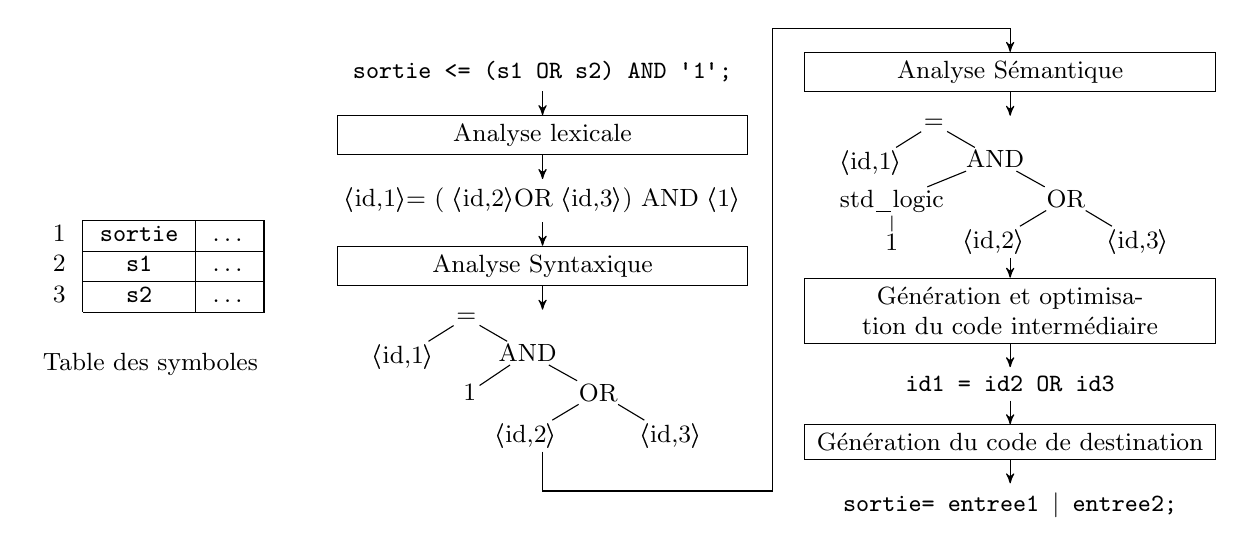
\begin{tikzpicture}[node font=\small, node distance = 0.3cm]
	\node[] (start) {\texttt{sortie <= (s1 OR s2) AND \textquotesingle 1\textquotesingle;}};
	\node[draw, text width = 5cm, text centered,below=of start] (lexical) {Analyse lexicale};
	\node[below=of lexical] (lexicalRes) {\textlangle id,1\textrangle  = ( \textlangle id,2\textrangle OR \textlangle id,3\textrangle ) AND \textlangle 1\textrangle };
	\node[draw, text width = 5cm, text centered,below=of lexicalRes] (Syntax) {Analyse Syntaxique};
	
	
	\begin{scope}[node distance=0.2 and 0.2cm, inner sep=1pt]
	\node[below left = 0.3cm and 0.8cm of Syntax.south] (SyntaxRes1) {=};
	\node[below left =of SyntaxRes1] (SyntaxRes11) {\textlangle id,1\textrangle};
	\node[below right =of SyntaxRes1] (SyntaxRes2) {AND};
	\node[below right =of SyntaxRes2] (SyntaxRes3) {OR};
	\node[below left =of SyntaxRes3] (SyntaxRes31) {\textlangle id,2\textrangle};
	\node[below right =of SyntaxRes3] (SyntaxRes32) {\textlangle id,3\textrangle};
	
	\node[below left = of SyntaxRes2] (SyntaxRes4) {1};
	
	
	\path[draw] (SyntaxRes1) -- (SyntaxRes2)
	(SyntaxRes1) -- (SyntaxRes11)
	(SyntaxRes2) -- (SyntaxRes3)
	(SyntaxRes2) -- (SyntaxRes4)
	(SyntaxRes3) -- (SyntaxRes31)
	(SyntaxRes3) -- (SyntaxRes32)
	;
	\end{scope}
	
	\node[draw, text width = 5cm, text centered,right = 0.8cm of start] (Semantic) {Analyse S\'emantique};
	%  \node[draw, text width = 5cm, text centered,anchor=north] (Semantic) at ($(Syntax.south |- SyntaxRes32.south) - (0,0.3cm)$) {Analyse S\'emantique};
	
	\begin{scope}[node distance=0.2 and 0.2cm, inner sep = 1pt]
	\node[below left =  0.3cm and 0.8cm of Semantic.south] (SemanticRes1) {=};
	\node[below left =of SemanticRes1] (SemanticRes11) {\textlangle id,1\textrangle};
	\node[below right =of SemanticRes1] (SemanticRes2) {AND};
	\node[below right =of SemanticRes2] (SemanticRes3) {OR};
	\node[below left =of SemanticRes3] (SemanticRes31) {\textlangle id,2\textrangle};
	\node[below right =of SemanticRes3] (SemanticRes32) {\textlangle id,3\textrangle};
	
	\node[below left = of SemanticRes2] (SemanticRes4) {std\_logic};
	\node[below = of SemanticRes4] (SemanticRes5) {1};
	
	
	\path[draw] (SemanticRes1) -- (SemanticRes2)
	(SemanticRes1) -- (SemanticRes11)
	(SemanticRes2) -- (SemanticRes3)
	(SemanticRes2) -- (SemanticRes4)
	(SemanticRes4) -- (SemanticRes5)
	(SemanticRes3) -- (SemanticRes31)
	(SemanticRes3) -- (SemanticRes32)
	;
	\end{scope}
	\node[draw,text width = 5cm, text centered, anchor=north] (codeIntGen) at ($(Semantic.south |- SemanticRes5.south) - (0,0.3cm)$) {G\'en\'eration et optimisation du code interm\'ediaire};
	\node[below=of codeIntGen] (codeIntGenRes) {\texttt{id1 = id2 OR id3}};
	\node[draw,text width = 5cm, text centered, below=of codeIntGenRes] (codeDestGen) {G\'en\'eration du code de destination};
	\node[below=of codeDestGen] (codeDestGenRes) {\texttt{sortie= entree1 \textbar ~entree2;}};
	
	
	\path[->,>=stealth'] (start) edge (lexical)
	(lexical) edge (lexicalRes)
	(lexicalRes) edge (Syntax)
	(Syntax) edge (Syntax.south |- SyntaxRes1.north)
	(Semantic) edge (Semantic.south |- SemanticRes1.north)
	(codeIntGen |- SemanticRes31.south) edge (codeIntGen)
	(codeIntGen) edge (codeIntGenRes)
	(codeIntGenRes) edge (codeDestGen)
	(codeDestGen) edge (codeDestGenRes) 
	;
	\path[->,>=stealth', draw]    (Syntax.south |- SyntaxRes31.south) |- 
	($(start.east |- SyntaxRes31.south) + (0.4,-0.5cm)$) |-
	($(start.east |- Semantic.north) + (0.4,0.3cm) $) -| 
	(Semantic.north)
	;
	\node[left=0.8cm of Syntax] (symbolTable) {
		\begin{tabular}{c|c|c|}
		\cline{2-3}
		1 & \texttt{sortie} & \ldots \\
		\cline{2-3}
		2 & \texttt{s1} & \ldots \\
		\cline{2-3}
		3 & \texttt{s2} & \ldots \\
		\cline{2-3}
		\end{tabular}
	};
	\node[below=of symbolTable] {Table des symboles};
	
	\end{tikzpicture}
	\caption{exemple}
\end{figure}

\todo[inline]{Mettre des trucs utiles}

\section{Conclusion}
On a bien travaillé

\end{document}          
